\documentclass{beamer}
\usepackage{listings}
\usepackage{color}
\usepackage{amsmath}
\usepackage{gvv}


\title{Equidistant Locus Problem}
\author{EE25BTECH11008 - Anirudh M Abhilash}
\date{September 12, 2025}

\begin{document}

%----------------- Title -------------------
\begin{frame}
\titlepage
\end{frame}

%----------------- Problem -------------------
\begin{frame}{Problem Statement}
Find a relation between $x$ and $y$ such that the point
\[
\vec{P}(x,y)
\]
is equidistant from
\[
\vec{A}(7,1), \quad \vec{B}(3,5).
\]
\end{frame}

%----------------- Solution -------------------
\begin{frame}{Solution}
Let 
\[
\vec{P} = \myvec{x \\ y}, \quad \vec{A} = \myvec{7 \\ 1}, \quad \vec{B} = \myvec{3 \\ 5}.
\]

Since $\vec{P}$ is equidistant from $\vec{A}$ and $\vec{B}$,
\[
\|\vec{P} - \vec{A}\| = \|\vec{P} - \vec{B}\|.
\]

Squaring both sides and using the inner product,
\begin{align}
(\vec{P} - \vec{A})^\top(\vec{P} - \vec{A}) &= (\vec{P} - \vec{B})^\top(\vec{P} - \vec{B}) \\[6pt]
\vec{P}^\top \vec{P} - 2\vec{P}^\top \vec{A} + \vec{A}^\top \vec{A} 
&= \vec{P}^\top \vec{P} - 2\vec{P}^\top \vec{B} + \vec{B}^\top \vec{B}.
\end{align}

Cancelling $\vec{P}^\top \vec{P}$,
\begin{align}
2\vec{P}^\top(\vec{B}-\vec{A}) &= \vec{B}^\top \vec{B} - \vec{A}^\top \vec{A}.
\end{align}

\end{frame}

\begin{frame}{Solution (cont..)}
Now,
\[
\vec{B} - \vec{A} = \myvec{3 \\ 5} - \myvec{7 \\ 1} = \myvec{-4 \\ 4}, 
\]
\[
\quad \vec{B}^\top \vec{B} = 3^2 + 5^2 = 34, 
\]
\[
\quad \vec{A}^\top \vec{A} = 7^2 + 1^2 = 50
\]

Thus,
\begin{align}
2\myvec{x & y}\myvec{-4 \\ 4} &= 34 - 50 \\[6pt]
-4x + 4y &= -8 \\[6pt]
y - x &= -2.
\end{align}

Hence, the required relation is
\[
\boxed{y = x - 2}
\]

\end{frame}

%----------------- Python Code -------------------
\begin{frame}[fragile]{Python Code}
\begin{lstlisting}[language=Python]

import numpy as np
import matplotlib.pyplot as plt

A = np.array([7, 1])
B = np.array([3, 5])

x_vals = np.linspace(0, 10, 100)
y_vals = x_vals - 2

plt.plot(x_vals, y_vals, 'k-')
plt.text(9, 6, r'y=x-2', fontsize=15)

\end{lstlisting}
\end{frame}

\begin{frame}[fragile]{Python Code(Cont..)}
\begin{lstlisting}[language=Python]
plt.scatter(*A, color='red')
plt.scatter(*B, color='blue')

plt.text(A[0]+0.3, A[1], 'A(7,1)')
plt.text(B[0]+0.3, B[1], 'B(3,5)')

plt.axhline(0, color='black', lw=0.5)
plt.axvline(0, color='black', lw=0.5)
plt.axis('equal')
plt.show()
\end{lstlisting}
\end{frame}

%----------------- C Code -------------------
\begin{frame}[fragile]{C Code}
\begin{lstlisting}[language=C]
#include <stdio.h>

void perpendicular_bisector(double x1, double y1,
                            double x2, double y2,
                            double *a, double *b,
                            double *c) {
    double mx = (x1 + x2) / 2.0;
    double my = (y1 + y2) / 2.0;

    double dx = x2 - x1;
    double dy = y2 - y1;

    *a = dx;
    *b = dy;
    *c = -((*a) * mx + (*b) * my);
}
\end{lstlisting}
\end{frame}

%----------------- Python + C -------------------
\begin{frame}[fragile]{Using C Code in Python}
\begin{lstlisting}[language=Python]
import ctypes, numpy as np, matplotlib.pyplot as plt

lib = ctypes.CDLL("./info.so")

lib.perpendicular_bisector.argtypes = (
    ctypes.c_double, ctypes.c_double,
    ctypes.c_double, ctypes.c_double,
    ctypes.POINTER(ctypes.c_double),
    ctypes.POINTER(ctypes.c_double),
    ctypes.POINTER(ctypes.c_double)
)

A, B = (7.0, 1.0), (3.0, 5.0)


\end{lstlisting}
\end{frame}
\begin{frame}[fragile]{Using C Code in Python(Cont..)}
\begin{lstlisting}[language=Python]
a = ctypes.c_double()
b = ctypes.c_double()
c = ctypes.c_double()

lib.perpendicular_bisector(A[0], A[1], B[0], B[1],
    ctypes.byref(a), 
    ctypes.byref(b), 
    ctypes.byref(c)
    )

x = np.linspace(0, 10, 100)
y = (-a.value*x - c.value)/b.value

plt.plot(x, y, 'k-', label='Bisector')

\end{lstlisting}
\end{frame}
\begin{frame}[fragile]{Using C Code in Python(Cont..)}
\begin{lstlisting}[language=Python]
plt.text(A[0] + 0.3, A[1], r'A(7,1)', fontsize=12, color='red')
plt.text(B[0] + 0.3, B[1], r'B(3,5)', fontsize=12, color='blue')
plt.text(7, ( -a.value*6 - c.value)/b.value + 0.3,
         f"{a.value:.0f}x+{b.value:.0f}y+{c.value:.0f}=0",
         fontsize=12, color="black")
plt.scatter(*A, color='red', label='A(7,1)')
plt.scatter(*B, color='blue', label='B(3,5)')
plt.axhline(0, color='gray', lw=0.5)
plt.axvline(0, color='gray', lw=0.5)
plt.legend()
plt.show()

\end{lstlisting}
\end{frame}

%----------------- Plots -------------------
\begin{frame}{Plot (Python)}
\centering
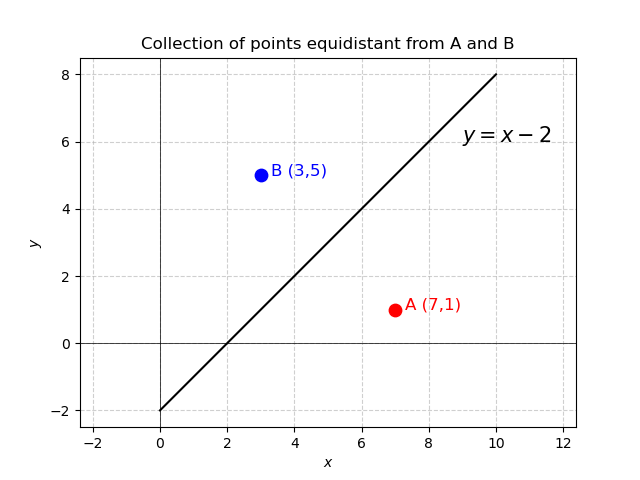
\includegraphics[width=0.8\linewidth]{figs/plt.png}
\end{frame}

\end{document}
